%
%% This is file `sample-sigconf.tex',
%% generated with the docstrip utility.
%%
%% The original source files were:
%%
%% samples.dtx  (with options: `sigconf')
%% 
%% IMPORTANT NOTICE:
%% 
%% For the copyright see the source file.
%% 
%% Any modified versions of this file must be renamed
%% with new filenames distinct from sample-sigconf.tex.
%% 
%% For distribution of the original source see the terms
%% for copying and modification in the file samples.dtx.
%% 
%% This generated file may be distributed as long as the
%% original source files, as listed above, are part of the
%% same distribution. (The sources need not necessarily be
%% in the same archive or directory.)
%%
%% Commands for TeXCount
%TC:macro \cite [option:text,text]
%TC:macro \citep [option:text,text]
%TC:macro \citet [option:text,text]
%TC:envir table 0 1
%TC:envir table* 0 1
%TC:envir tabular [ignore] word
%TC:envir displaymath 0 word
%TC:envir math 0 word
%TC:envir comment 0 0
%%
%%
%% The first command in your LaTeX source must be the \documentclass command.
\documentclass[sigconf,nonacm]{acmart}
%% NOTE that a single column version may be required for 
%% submission and peer review. This can be done by changing
%% the \doucmentclass[...]{acmart} in this template to 
%% \documentclass[manuscript,screen]{acmart}
%% 
%% To ensure 100% compatibility, please check the white list of
%% approved LaTeX packages to be used with the Master Article Template at
%% https://www.acm.org/publications/taps/whitelist-of-latex-packages 
%% before creating your document. The white list page provides 
%% information on how to submit additional LaTeX packages for 
%% review and adoption.
%% Fonts used in the template cannot be substituted; margin 
%% adjustments are not allowed.
%%
%%
%% \BibTeX command to typeset BibTeX logo in the docs


%% Rights management information.  This information is sent to you
%% when you complete the rights form.  These commands have SAMPLE
%% values in them; it is your responsibility as an author to replace
%% the commands and values with those provided to you when you
%% complete the rights form.
\setcopyright{acmcopyright}
\copyrightyear{2022}
\acmYear{2022}


%% These commands are for a PROCEEDINGS abstract or paper.

%
%  Uncomment \acmBooktitle if the title of the proceedings is different
%  from ``Proceedings of ...''!
%
%\acmBooktitle{Woodstock '18: ACM Symposium on Neural Gaze Detection,
%  June 03--05, 2018, Woodstock, NY} 



%%
%% Submission ID.
%% Use this when submitting an article to a sponsored event. You'll
%% receive a unique submission ID from the organizers
%% of the event, and this ID should be used as the parameter to this command.
%%\acmSubmissionID{123-A56-BU3}

%%
%% For managing citations, it is recommended to use bibliography
%% files in BibTeX format.
%%
%% You can then either use BibTeX with the ACM-Reference-Format style,
%% or BibLaTeX with the acmnumeric or acmauthoryear sytles, that include
%% support for advanced citation of software artefact from the
%% biblatex-software package, also separately available on CTAN.
%%
%% Look at the sample-*-biblatex.tex files for templates showcasing
%% the biblatex styles.
%%

%%
%% The majority of ACM publications use numbered citations and
%% references.  The command \citestyle{authoryear} switches to the
%% "author year" style.
%%
%% If you are preparing content for an event
%% sponsored by ACM SIGGRAPH, you must use the "author year" style of
%% citations and references.
%% Uncommenting
%% the next command will enable that style.
%%\citestyle{acmauthoryear}



\usepackage{verbatim}
\usepackage{graphicx}
\usepackage{adjustbox}
\usepackage[linesnumbered, boxed, resetcount]{algorithm2e}

%%
%% If you need any other LaTeX packages, add them here
%%

%%
%% end of the preamble, start of the body of the document source.
\begin{document}

%%
%% The "title" command has an optional parameter,
%% allowing the author to define a "short title" to be used in page headers.
\title{Artificial intelligence in game 2048}


%%
%% The "author" command and its associated commands are used to define
%% the authors and their affiliations.
%% Of note is the shared affiliation of the first two authors, and the
%% "authornote" and "authornotemark" commands
%% used to denote shared contribution to the research.
\author{Maj Gaber\v{s}\v{c}ek}
%\authornote{All three authors contributed equally to this research.}
\email{mg5781@student.uni-lj.si}
\affiliation{%
    \institution{Faculty of Mathematics and Physics,\\
    University of Ljubljana \\Jadranska ulica 19}
    \city{SI-1000 Ljubljana}
    \country{Slovenia}
}

\setcopyright{iw3c2w3}

%%
%% The abstract is a short summary of the work to be presented in the
%% article.
\begin{abstract}
    I implemented a simple game of 2048 along with user interface in programming language Java. Along with single player option to play the game, I also implemented some algorithms, which try to solve the game. All algorithms have a different fundation, some base on positional play (position evaluator) and some are based on Monte Carlo methods (simulator and dynamic simulator). Overall, I would say that best algorithm is dynamic simulator, as it best compensates between move time and success. 
\end{abstract}

%%
%% Keywords. The author(s) should pick words that accurately describe
%% the work being presented. Separate the keywords with commas.
\keywords{2048, puzzle game, artificial intelligence, problem solving, Monte Carlo methods, algorithms}

%%
%% This command processes the author and affiliation and title
%% information and builds the first part of the formatted document.
\maketitle

\section{Introduction}

I have played the game 2048 and been a fan of it ever since high school. The game is quite simple, however it requires smart planning in order to beat it. Since I haven't found many articles, that describe algorithms, which are successful at playing the game, I decided to implement some methods myself. The goal was to find different types of algorithms, that are all fairly good at playing the game. Of course, all the algorithms have to make a move reasonably fast.

\section{About 2048}

2048 is a single player video game, invented by an italian software developer Gabriele Cirulli as a weekend project and later published on \texttt{Github}. The goal of the game is to merge smaller numbers on the board in order to reach higher numbers (or more specifically, 2048). Some variantations of the game of course also allow infinite play, so that the game tries to reach higher numbers. The board is usually of size 4x4, but there are many different variantations as well (3x3, 5x5 or even 8x8). \cite{wiki:2048_(video_game)}

The game is not deterministic and it involves probability. Therefore it is important to understand, that theoretically, even if played perfectly, there exists a probability that the game will be lost. With a reduction to 3-SAT problem, it has been proved that the problem of 2048 is NP-complete \cite{DBLP:journals/corr/AbdelkaderAD15}.

\section{Algorithms}

This section of the article describes all the algorithms and how they work.

\subsection{Random moves algorithm}

First algorithm is very simple. It is playing completely random moves, no matter the position. This algorithm is not very good at solving the game, however it serves as a base for \textit{Simulator} and \textit{Dynamic simulator} algorithms, which are described later.

\subsection{Empty spaces algorithm}

Another simple algorithm checks all the moves and plays the one, that results in most empty board. If more moves result in the same number of empty spaces, a certain move priority is specified. This algorithm is of course too simple to achieve anything. However, the its main goal was to analyse, how much better then simple random moves it can be. 

\subsection{Position evaluator algorithm}

The position evaluating algorithm contains a parameter of depth. It uses depth first search and searches all the possible positions for the specified depth. Then it evaluates all the positions and plays the move, that results in best expected position evaluation. The problem with this is, that because a new number is spawned to a random position on a board after each move, the breaching factor is very big. So realistically, we can only use depth 2.

\begin{figure}[!ht]
    \centering
    \begin{adjustbox}{scale=0.35}
    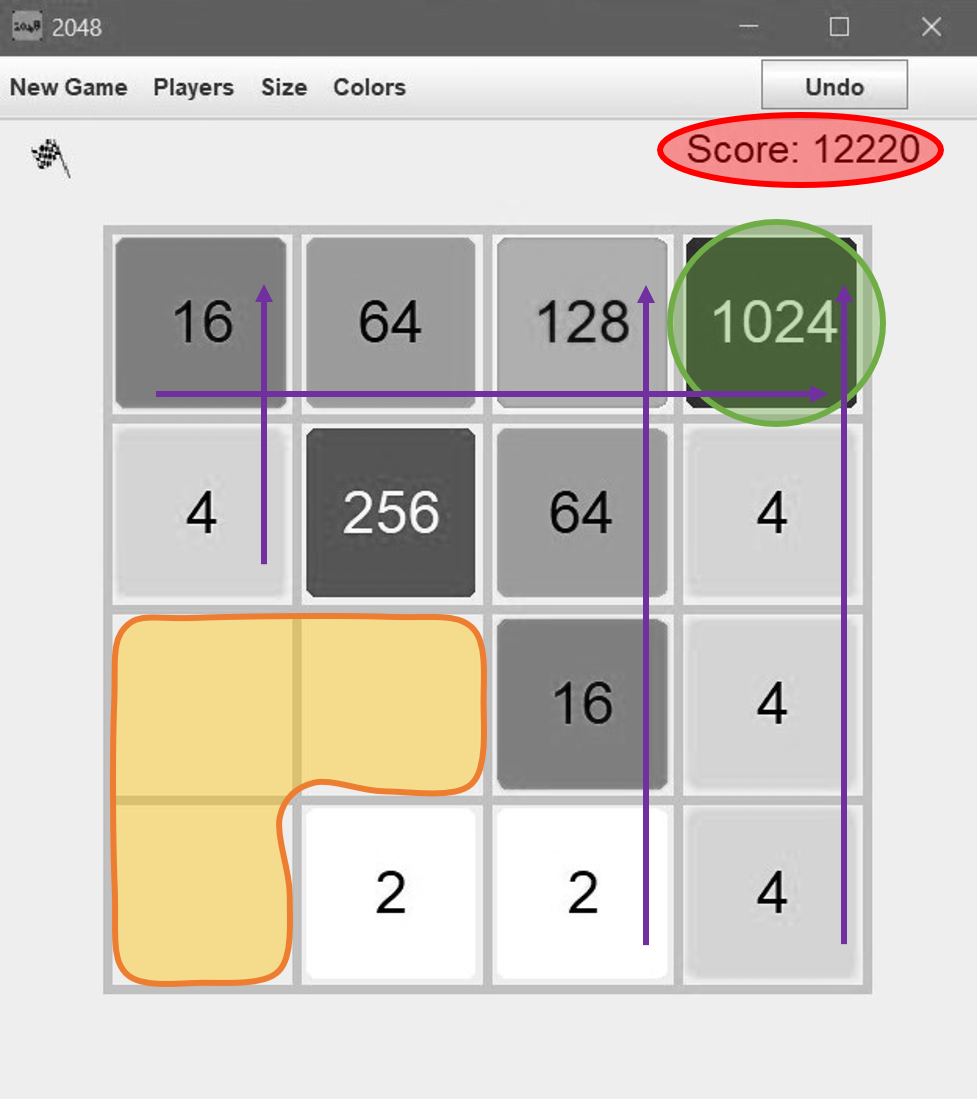
\includegraphics{static/evaluator.png}
    \end{adjustbox}
    \caption{Visualization of position evaluation}
    \label{fig:evaluator}
\end{figure}

Position evaluation explanation is visualized in Figure \ref{fig:evaluator}. First contributor towards evaluation is the score of the game (color red). By doing this, we force the game to merge bigger tiles as fast as possible. Second contributor towards evaluation is the most important one. We always check if the tile with the biggest number is in the top right corner (green color). Then we check first row and every column. If they are ordered (in the direction of the purple arrow), it further contributes towards position score. Number of empty spaces also affect the evaluation of the position.

\subsection{Simulator and dynamic simulator}

This algorithm is well known in Game theory as \textbf{Pure Monte Carlo game search}. Algorithm has input integer $k$. Then it looks for all possible moves in the given position.
For each of this moves, it then plays the move and simulates rest of the game (until game over) with the \textit{Random moves algorithm}. It does this $k$ times for each possible move and returns a move, that averages highest game score across $k$ games.

The only problem with Simulator is, that for bigger $k$, not only performance increases, but also move time. So we want as small $k$ as possible, for which the algorithm still successfully plays. After some testing, I found out, that algorithm only has trouble right before building another biggest number. That is because right before building, for example 1024, there must be a 512, 256, 128, 64, 32, 16, 8, 4 and double 2 already on the board.

So, to optimize move time and success combination, I introduced another algorithm, which dynamically changes $k$, based on the game's score. If the score indicates, that we are about to reach a complex position (as described above), it increases $k$. Otherwise, we compromise $k$ and rather focus on playing as fast as possible. $k$ in regard to score is visualized in Figure \ref{fig:dynamic_depth}.

\begin{figure}[!ht]
    \centering
    \begin{adjustbox}{scale=0.45}
    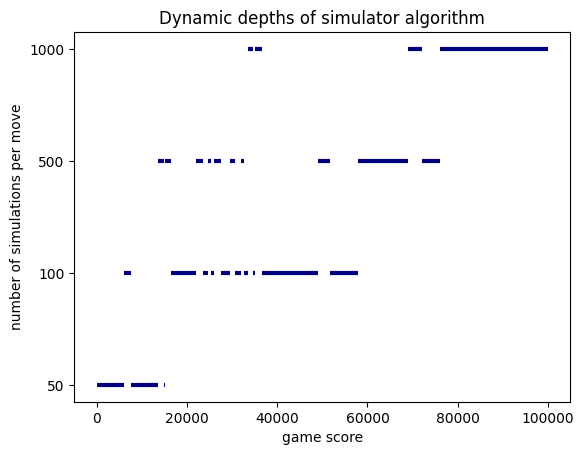
\includegraphics{static/dynamic_sim.png}
    \end{adjustbox}
    \caption{Depth in regard to score for dynamic simulator algorithm}
    \label{fig:dynamic_depth}
\end{figure}

\section{Evaluation of algorithms}

Of course the main evaluation of the algorithms has to be percentage of winning, which is shown in Figure \ref{fig:win_perc}. Best is Simulator with $k=500$, but dynamic simulator is far faster and almost equally successful.

\begin{figure}[!ht]
    \centering
    \begin{adjustbox}{scale=0.45}
    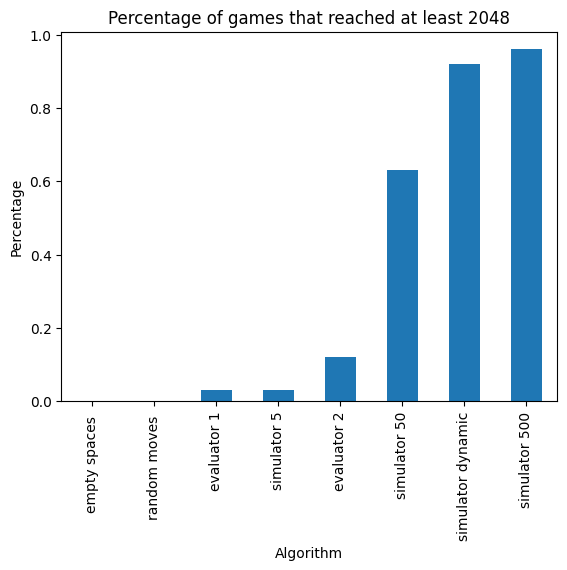
\includegraphics{static/percentage_of_wins.png}
    \end{adjustbox}
    \caption{Percentage of times that algorithm reached 2048}
    \label{fig:win_perc}
\end{figure}

In the Figure \ref{fig:dist_of_highest}, we can see distribution of highest number reached (before losing) of each algorithm. This provides more insight into Evaluator algorithm of depth 2. It seems to reach at least 1024 most of the times, but then fails to reach 2048.

\begin{figure}[!ht]
    \centering
    \begin{adjustbox}{scale=0.45}
    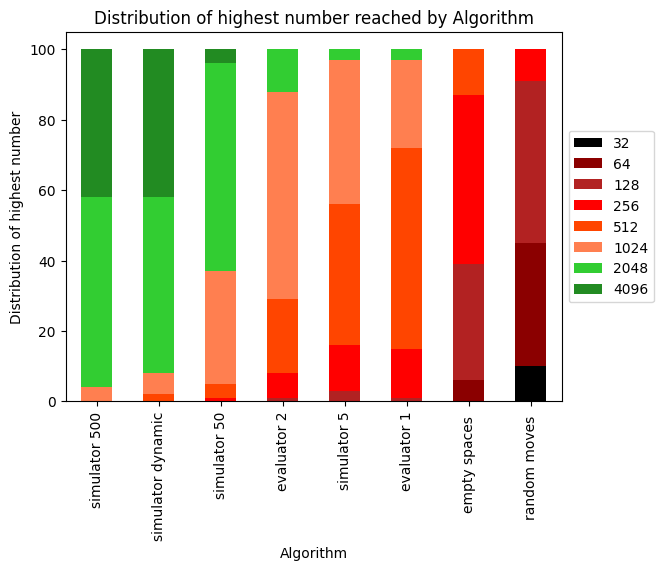
\includegraphics{static/distribution_of_highest_reached.png}
    \end{adjustbox}
    \caption{Distribution of highest reached tile when losing}
    \label{fig:dist_of_highest}
\end{figure}

\section{Conclusions}

Overall, I think that best algorithm is the Dynamic simulator. However, the position evaluator's playstyle very much imitates how humans plays the game. If parameters of this algorithm (for position evaluation) would be better tuned or they could dynamically change (in regard to score), winning chances could increase. This is one of the further work possibilities. 


\bibliographystyle{ACM-Reference-Format}
\bibliography{references}

\end{document}
